This section describes the purpose, use, and intended user audience for the RV8 Work Cell. RV8 Work Cell is a system that performs precise marking using an air brush in an industrial manner. Users of this work cell will be able to practice standards in industrial robotics, while improving time efficiency. 
\subsection{Purpose and Use}
The conventional approach to automotive air brushes in warehouses contains several challenges. Using manual spray painting or air brush for painting can be time consuming, and can cause errors in its precision. Since manual spray painting can be prone to errors, any imprecise markings can cause cost overheads due to cleaning and repainting on the product. Finally, with modern commerce continuing to grow, spray painting on different products must be done with efficiency, while saving time and costs per paint. The RV8 robot work cell will precisely paint using an air brush in an organized manner according to customer's requirements with high efficiency and accuracy.

\subsection{Intended Audience}
This product is considered industrial, so the intended audience of this product are warehouses and factories where manual labor can be automated through the use of robotics.

\begin{figure}[h!]
	\centering
   	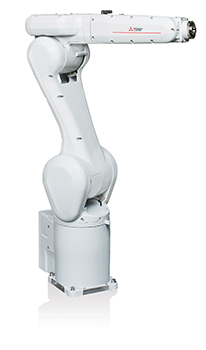
\includegraphics[width=0.40\textwidth]{images/rv8crl.jpeg}
    \caption{Mitsubishi RV8-CRL  \cite{MitsubishiRV8CRL}}
\end{figure}
